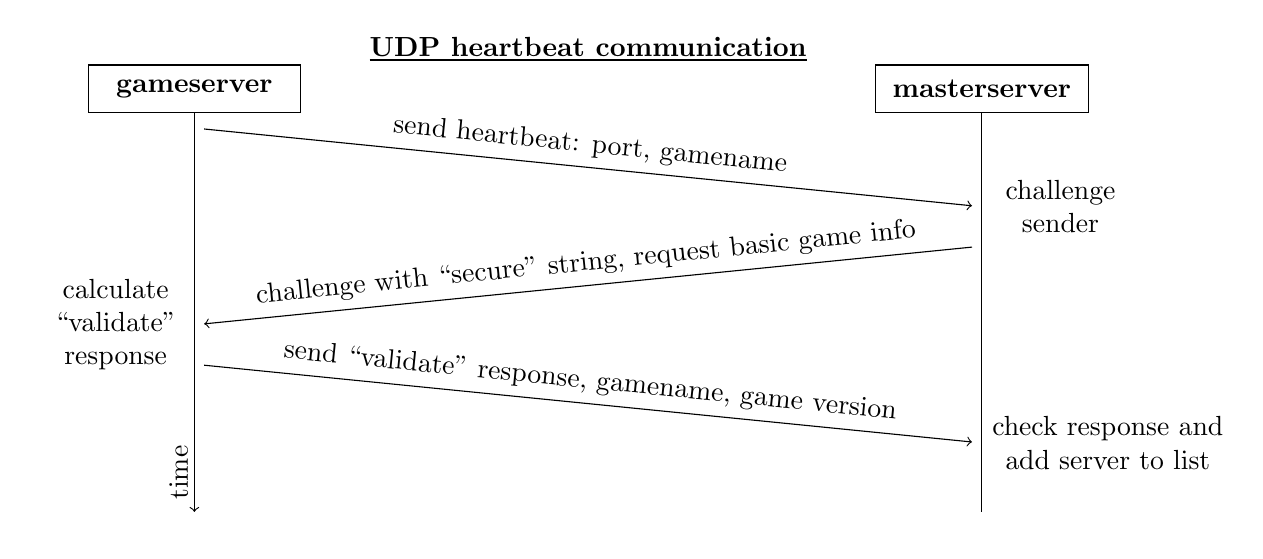
\begin{tikzpicture}

% figure title
\node[rectangle] at (5, 6) (title) {\underline{\bf UDP heartbeat communication}};

% gameserver and masterserver
\node[draw, rectangle, minimum height=0.6cm, minimum width=2.7cm] at ( 0, 5.5) (gstop) {\bf gameserver};
\node[draw, rectangle, minimum height=0.6cm, minimum width=2.7cm] at (10, 5.5) (mstop) {\bf masterserver};

% heartbeat
\node at ( 0,  5) (gshb) {};
\node at (10,  4) (mshb) {};
\node at (11,  4) (mssecure) [text width=2cm,text centered]{challenge\\sender};
\draw[->] (gshb) -- (mshb) node[midway, above, sloped] {send heartbeat: port, gamename};

% secure challenge
\node at (10,  3.5) (msse) {};
\node at ( 0,  2.5) (gsse) {};
\node at (-1,  2.5) (msvalidate) [text width=2cm,text centered]{calculate\\``validate''\\response};
\draw[->] (msse) -- (gsse) node[midway, above, sloped] {challenge with ``secure'' string, request basic game info};

% validate        
\node at ( 0,  2) (gsva) {};
\node at (10,  1) (msva) {};
\node at (11.6,  1) (mscmp) [text width=3cm, text centered]{check response and add server to list};
\draw[->] (gsva) -- (msva) node[midway, above, sloped] {send ``validate'' response, gamename,  game version};

% gameserver and masterserver bottom, vertical lines
\node at ( 0, 0) (gsbot) {};
\node at (10, 0) (msbot) {};
\draw[->] (gstop.270) -- (gsbot.90) node[at end, xshift=-0.2cm, yshift=0.5cm, rotate=90] {time};
\draw (mstop.270) -- (msbot.90) {};

\end{tikzpicture}
